\begin{exercise}{trigonometrie.dreieck.im.dreieck}{Dreieck im Dreieck}
  \ifproblem\problem\par
    \begin{minipage}{0.29\textwidth}
      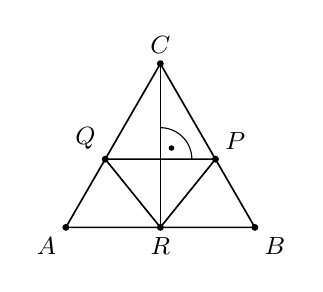
\begin{tikzpicture}
        % Punktkoordinaten
        \coordinate (A) at ( 0.0000,  0.0000);
        \coordinate (B) at ( 2.4000,  0.0000);
        \coordinate (C) at ( 1.2000,  2.0785);
        \coordinate (P) at ( 1.9000,  0.8660);
        \coordinate (Q) at ( 0.5000,  0.8660);
        \coordinate (R) at ( 1.2000,  0.0000);
        \coordinate (M) at ( 1.2000,  0.8660);
        % Seiten der Dreiecke
        \draw[line width=0.6pt] (A) -- (B) -- (C) -- cycle;
        \draw[line width=0.6pt] (P) -- (Q) -- (R) -- cycle;
        % Hoehe
        \draw[line width=0.6pt] (C) -- (R);
        % Punkte
        \fill (A) circle[radius=1.25pt];
        \fill (B) circle[radius=1.25pt];
        \fill (C) circle[radius=1.25pt];
        \fill (P) circle[radius=1.25pt];
        \fill (Q) circle[radius=1.25pt];
        \fill (R) circle[radius=1.25pt];
        % rechter Winkel
        \begin{scope}
          \clip (M) -- (P) -- (C) -- cycle;
          \draw (M) circle[radius=0.4];
          \fill ([shift={(45:0.2)}]M) circle[radius=1pt];
        \end{scope}
        % Beschriftung
        \node[below left]  at (A) {{\small$A$}};
        \node[below right] at (B) {{\small$B$}};
        \node[above]       at (C) {{\small$C$}};
        \node[above right] at (P) {{\small$P$}};
        \node[above left]  at (Q) {{\small$Q$}};
        \node[below]       at (R) {{\small$R$}};
      \end{tikzpicture}
    \end{minipage}%
    \hfill
    \begin{minipage}{0.70\textwidth}
      Einem gleichseitigem Dreieck $\triangle ABC$ mit
      $\overline{AB}=\SI{12}{\centi\metre}$ wird ein
      Dreieck $\triangle PQR$ so einbeschrieben, dass
      die Seite $\overline{PQ}$ eine Länge von
      \SI{7}{\centi\metre} besitzt.\par
      Berechne den Flächeninhalt des einbeschriebenen
      Dreiecks $\triangle PQR$ und die Schenkellänge
      $\overline{QR}$.
    \end{minipage}%
  \fi
  %\ifoutline\outline\par
  %\fi
  %\ifoutcome\outcome\par
  %\fi
\end{exercise}
